\iffalse
\begin{itemize}
	\item Initial state construction (State Identification)
	\item Aggregation (State Aggregation)
	\item Transition probabililties (Modeling transitions)
\end{itemize}
\fi

The key idea at the heart of our system is to build and visualize an abstraction of the underlying 
dynamics of the system. Our abstraction is based on Markov chains where we represent the dynamics of the data using states and transitions. A key feature of our system is \lstopar{to} present this abstraction over \emph{multiple scales}. 
%
%To capture and summarize the dynamics of the system our methodology represents the data
%in a qualitative manner using states and transitions. 
%
We begin by presenting an overview
of our multi-scale methodology. The methodology consists of four main steps as shown in Figure \ref{fig:methodology}.
\begin{figure*}[]
	\centering
	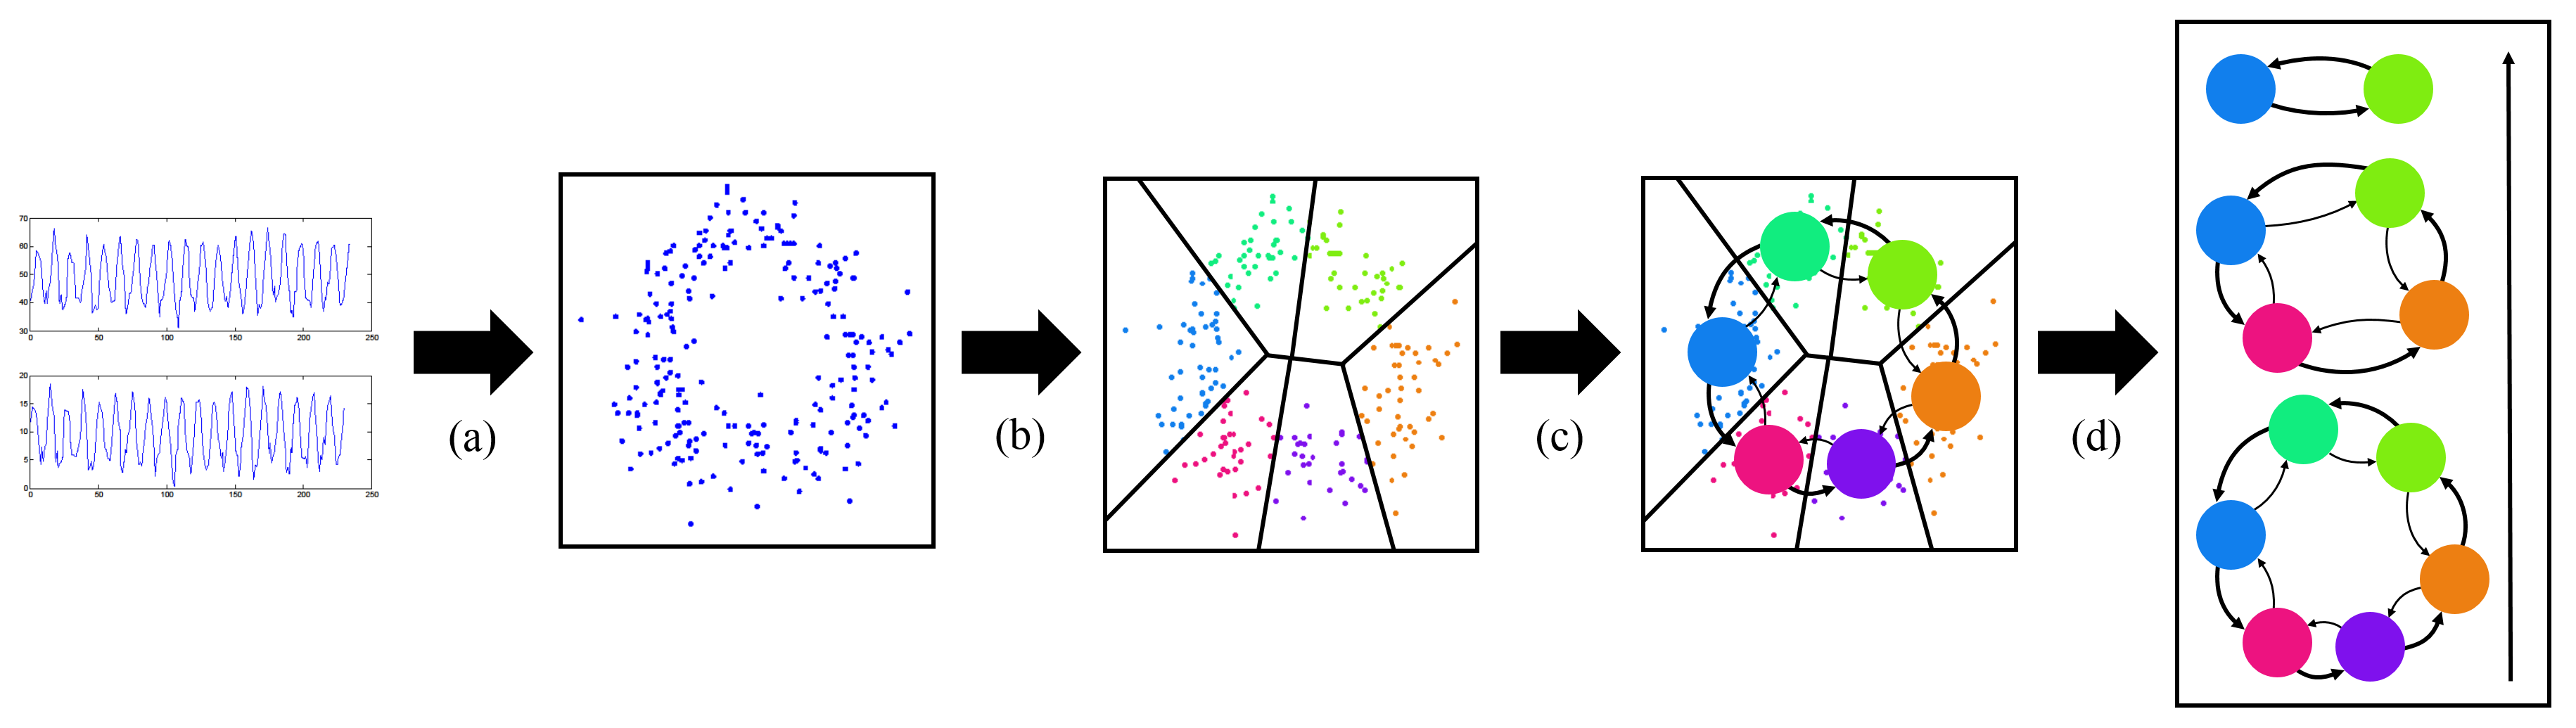
\includegraphics[width=\textwidth]{methodology-V2-fixed}
	\caption{Overview of the proposed three-step methodology.}
	\label{fig:methodology}
\end{figure*}

We begin by considering the multivariate time series as a point cloud in high dimensional space, ignoring the time component. The second step identifies the underlying structure of this point cloud, identifying their most typical states. In Figure~\ref{fig:methodology}, we see two noisy periodic signals which are partitioned roughly according to the phase of the system. As described in Section \lstopar{\ref{} xxx}, this is done by considering a metric on the data points and partitioning or clustering them. Each cluster/partition is then associated to a state in a Markov model. We refer to these as the low level states. The 
 dynamics are modeled through the transition probabilities between the states using continuous time Markov chains (Section \ref{sec:preliminaries}). Finally, we construct a hierarchy of such Markov chains by aggregating the initial states into coarser states. Each level of the hierarchy is associated to a unique scale, yielding a multi-scale model.

%The methodology starts in the top left part of the figure with an initial step that summarizes
%the structure of the data by identifying their most typical states. It achieves this by \lstopar{placing}
%the data in a \lstopar{design time} metric space and partitioning them. It then associates
%each partition with a single state.
% \lstopar{
% \begin{itemize}
% 	\item These states are used as the lowest-level states.
% \end{itemize}
% }
%In the second step we summarize dynamics by modeling transition probabilities using continuous time Markov chain framework presented in Section \ref{sec:preliminaries}.
% The third and final step aggregates states and transitions into a hierarchy, associating each
% level of the hierarchy with a unique scale, thus providing a multi-scale model. These steps 
% are explained in detail in the following subsections.


% \subsection{Initial State Construction}
% \label{sec:framework-states}

To construct the initial low level states, we define a partition function $\lstopar{f}: \mathbb{R}^d \rightarrow I$ mapping the $d$-dimensional signal to a finite, discrete set $I$. These represent the states which represent the basic unit of abstraction in our visualization. To complete the construction of the continuous-time Markov chain, we must define the transition rates.

%The first step in our methodology is the construction of initial lowest level states. Using the notation
%from Section \ref{sec:preliminaries} we define a partition function 
%from $\lstopar{f}: \mathbb{R}^d \rightarrow I$ mapping the $d$-dimensional signal to lowest level states
% \lstopar{
% with the following properties:
% \begin{itemize}
% 	\item similar points in $\mathbb{R}^d$ should be mapped to the same or neighboring partitions.
% \end{itemize} 
% }

%\subsection{Modeling Transition Probabilities}
%\label{sec:framework-transitions}

%While we represent the states as described in Section \ref{sec:framework-states},
Recall that all the data needed to represent a continuous-time Markov chain
is stored as transition rates in a transition rate matrix $Q \in \mathbb{R}^{n \times n}$, where $n$ represents
the cardinality of the finite state space $I$ (Section \ref{sec:preliminaries}). However, initial user
feedback showed that transition rates are not a very informative way of visualizing state transitions. Instead, 
we choose to visualize transitions in terms of the jump chain $\Pi$.
This represents an alternative, but equivalent, representation of a Markov chain by its jump chain and holding times. 

The jump chain of a continuous time Markov chain $(X_t)_{t \ge 0}$ is
a discrete time Markov chain $(Y_n)_{n \ge 0}$ with transition matrix $\Pi$ defined as
\begin{equation}
	\nonumber
	\left(\Pi\right)_{ij} = 
		\left\{
			\begin{array}{ll}
				-\frac{q_{ij}}{q_{ii}} & \mbox{if } i \ne j, q_{ii} \ne 0 \\
				0 & \mbox{if } i \ne j, q_{ii} = 0
			\end{array}
		\right.
\end{equation}
\begin{equation}
	\nonumber
	\left(\Pi\right)_{ii} = 
		\left\{
			\begin{array}{ll}
				0 & \mbox{if } q_{ii} \ne 0 \\
				1 & \mbox{if } q_{ii} = 0
			\end{array}
		\right.
\end{equation}

The formal definition of a Markov chain in terms of its jump chain and holding times is given belows.
\begin{defn}
	\label{def:jump-chain-holding-times}
	A right-continuous process $(X_t)_{t \ge 0}$ is a continuous time Markov chain with initial
	distribution $\lambda$ and transition rate matrix $Q$ if its jump chain $(Y_n)_{n \ge 0}$ is a 
	discrete time Markov chain with initial distribution $\lambda$ and transition matrix $\Pi$ and
	for each $n \ge 1$, conditional on $Y_0, Y_1, ..., Y_{n-1}$, its holding times $S_1, S_2, ..., S_{n-1}$
	are independent exponentially distributed random variables of parameters $q_{Y_0}, q_{Y_1}, ..., q_{Y_{n-1}}$
	where $q_i = -q_{ii}$.
\end{defn}

The states and jump matrix define a directed graph which we use to visualize the system. The widths of the arrows represent the corresponding values of the jump matrix. This only encodes the state transitions. To visualize how long the system spends in a state, we use the size of the state.
To determine the size of each state, we turn to the ergodic properties of $(X_t)_{t \ge 0}$. Specifically
we use the elements of the stationary distribution $\pi = (\pi_1, \pi_2, ..., \pi_n)$ and draw the area of
state $i$ proportional to $\pi_i$. We note that under the assumptions presented in Section \ref{sec:preliminaries}
this distribution always exists. \primoz{why do we not use the holding times  - a sentence or two here} \lstopar{we don't use them, we only use the jump chain. It would be possible to use the holding times as to calcualte the state radius.}

\lstopar{Actually we do use in a tooltip to show how long the systems stays in a state upon arrival.
\begin{equation}
	\nonumber E(T_i) = \frac{1}{q_i}
\end{equation}
where $T_i$ is the $i$-th states' holding time.
}

\subsection{Aggregation}
\label{sec:framework-aggregation}

One of the main contributions of this paper is to visualize the system at multiple scales  representing
the data at different detail levels - from the finest to the coarsest. To build our multi-scale representation we take as input, the continuous time Markov chain, we initially constructed. 

Recall from Section \ref{sec:preliminaries}, rather than constructing a single partition of our space, we can construct a hierarchical partition. With this hierarchical partition,  each scale $s$ is associated with a specific partition
function $\lstopar{f_s}: \mathbb{R}^d \rightarrow \lstopar{I_s}$. At the finest scale, we use the partition function \lstopar{$f: \mathbb{R}^d \rightarrow I$}, defined above, inducing state space $I$ of Markov chain $(X_t)_{t \ge 0}$. 
We then compute \lstopar{$f_s$} by aggregating elements of $I$ using mapping \lstopar{(projection?, parition?)} $\phi_s: I \rightarrow I_s$ and representing \lstopar{$f_s$} as a composition $\lstopar{f_s} = \lstopar{f} \circ \phi_s$. \textcolor{red}{$\phi_s$ is defined using $P_{\phi_s}$} 
\lstopar{
\begin{itemize}
	\item now we have defined everything we need to calcualte the new Markov chain $(X_t^s)_{t \ge 0}$: $f$ and $\phi_s$
\end{itemize}
}

All that remains is to compute the transition rate matrix of the new Markov chain $(X_t^{s})_{t \ge 0}$ induced \lstopar{by} state space $I_s$. To do so, we adapt the formula proposed in \cite{5746509} to continuous time Markov chains. We define function $\Phi_s: \mathbb{R}^{n \times n} \rightarrow \mathbb{R}^{m \times m}$ with $m \le n$ as:
\begin{equation}
	\label{eq:ctmc-state-aggregation}
	\Phi_s(Q) = (P_{\phi_s}' \Pi P_{\phi_s})^{-1} P_{\phi_s}' \Pi Q P_{\phi_s}
\end{equation}
where $\Pi = diag(\pi)$, $\pi$ is the stationary distribution of $(X_t)_{t \ge 0}$ and $P_{\phi_s}$ is a 
$n \times m$ matrix with elements
\begin{equation}
	\nonumber
	\left(P_{\phi_s}\right)_{ij} = 
		\left\{
			\begin{array}{ll}
				1 & \mbox{if } \phi_s(i) = j \\
				0 & \mbox{otherwise}.
			\end{array}
		\right.
\end{equation}

%We then compute the partition function $f_s: \mathbb{R}^d \rightarrow I_s$ for coarser scales by aggregating elements of $I$, \lstopar{inducing} state space $I_s$. Thus $I_s$ represents a partition of $I$ and can again be used as the state space on scale $s$. $I_s$ is determined by a map $\phi_s: I \rightarrow I_s$. This way $f_s$, can be represented as \lstopar{$f_s = f \circ \phi_s$}.

%The details of how compute $\lstopar{f}$ and $\phi_s$ are described in Section~\ref{}. Therefore, the problem is given $I$, $I_s$, $f$ and the Markov chain induced by $I$, to compute the Markov chain induced by $I_s$.

%Therefore given $\lstopar{f}$ and $\phi_s$ we have all the information to construct a new Markov chain $(X_t^{(s)})_{t \ge 0}$, induced by state space $I_s$. All that remains is to compute the corresponding transition rate matrix $Q^{(s)}$. To do so, we adapt the formula proposed in \cite{5746509} to continuous time Markov chains. We define function $\Phi_s: \mathbb{R}^{n \times n} \rightarrow \mathbb{R}^{m \times m}$ with $m \le n$ using formula~\ref{eq:ctmc-state-aggregation}.

%The states of this new Markov chain $(X_t^{(s)})_{t \ge 0}$ are induced by $I_s$, what remains is to compute the corresponding  transition rate matrix $Q^{(s)}$. To compute $Q^{(s)}$, we adapt the formula proposed in \cite{5746509} to continuous time Markov chains. We define function $\Phi_s: \mathbb{R}^{n \times n} \rightarrow \mathbb{R}^{m \times m}$ with $m \le n$ using formula~\ref{eq:ctmc-state-aggregation}.
%\begin{equation}
%	\label{eq:ctmc-state-aggregation}
%	\Phi_s(Q) = (P_{\phi_s}' \Pi P_{\phi_s})^{-1} P_{\phi_s}' \Pi Q P_{\phi_s}
%\end{equation}
%where $\Pi = diag(\pi)$, $\pi$ is the stationary distribution of $(X_t)_{t \ge 0}$ and $P_{\phi_s}$ is a 
%$n \times m$ matrix with elements
%\begin{equation}
%	\nonumber
%	\left(P_{\phi_s}\right)_{ij} = 
%		\left\{
%			\begin{array}{ll}
%				1 & \mbox{if } \phi_s(i) = j \\
%				0 & \mbox{otherwise}.
%			\end{array}
%		\right.
%\end{equation}
Thus the data needed to represent a Markov chain at a specific scale $s$ is obtained as $Q^{(s)} = \Phi_s(Q)$.
If we define $\psi_s = \phi_s \circ \phi_s^{-1}$, then Equation \ref{eq:ctmc-state-aggregation} can be rewritten as
\begin{equation}
	\label{eq:ctmc-aggregation-alternative}
	q_{\phi_s(i)\phi_s(j)}^{(s)} = \frac{\sum_{k \in \psi_s(i)}\pi_k \sum_{l \in \psi_s(j)} q_{kl}}{\sum_{k \in \psi_s(i)}\pi_k}
\end{equation}
$\pi^{(s)}$, the stationary distribution of $(X_t^{s})_{t \ge 0}$, can be computed directly from
the stationary distribution of the original chain $(X_t)_{t \ge 0}$ by the following rule:
\begin{equation}
	\nonumber
	\pi^{(s)} = \pi P_{\phi_s}.
\end{equation}
Intuitively, the stationary distributions are preserved through the scales, although the intermediate dynamics may change. How much, depends on how we construct our hierarchical partition function. 

\primoz{why not just recompute - we need a sentence here} \lstopar{ - it's slower, you need an iterative procedure to compute the stationary distribution}
